%!TEX TS-program = xelatex
\documentclass[]{friggeri-cv}
\usepackage{afterpage}
\usepackage{fontawesome}
\usepackage{hyperref}
\usepackage{color}
\usepackage{xcolor}
\usepackage{multirow}
\usepackage{array}
\usepackage{tabu}
\hypersetup{
    pdftitle={},
    pdfauthor={},
    pdfsubject={},
    pdfkeywords={},
    colorlinks=false,       % no link border color
    allbordercolors=white   % white border color for all
}
\RequirePackage{xcolor}
\definecolor{darkred}{HTML}{9F033B}

\begin{document}
\header{Danielle }{O'Sullivan}
      {\-\hspace{-1.9cm} Software Engineer | Accenture}
      
% Fake text to add separator      
\fcolorbox{white}{black}{\parbox{\dimexpr\textwidth-2\fboxsep-2\fboxrule}{%
.....
}}

% In the aside, each new line forces a line break
\begin{aside}
    %\section{} % Photo
        %{\includegraphics[scale=0.1]{img/circledp.png}}
    %~
    \section{Address}
        84 Vida House
        50 Trundleys Road
        London
        SE8 5EJ
    ~
    \section{Contact}
        07935 117 254
        \href{mailto:danielle.oh.es@gmail.com}{\textbf{danielle.oh.es@}\\gmail.com}
    ~
    \section{Social}
        \href{https://www.linkedin.com/in/danielleosullivan}danielleosullivan {\includegraphics[scale=0.015]{img/linkedin.jpg}}
        \href{https://github.com/danielleos}danielleos {\includegraphics[scale=0.025]{img/github.png}}
        \href{http://danielleosullivan.com}{\textbf{danielleosullivan.com}}
    ~
    \section{Programming}
        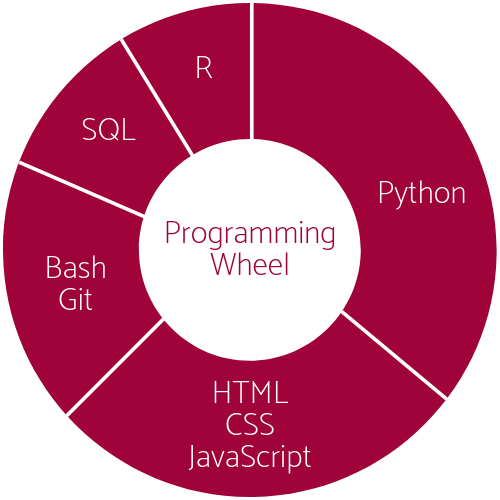
\includegraphics[scale=0.25]{img/programmingwheel.png}
    ~
    \section{Languages}
        \textbf{English}\includegraphics[scale=0.40]{img/5stars.png}
        \textbf{Spanish}\includegraphics[scale=0.40]{img/3stars.png}
        \textbf{Japanese}\includegraphics[scale=0.40]{img/2stars.png}
    ~
    \section{Sport}
        \textbf{Taekwon-Do}:
        \textbf{Blue Belt}\\5 gold, 4 silver, 3 bronze
        National level 2014-16
    ~
    \section{References}
        \textbf{Sudhir Sarangapany}
        Principal IT Solutions Architecture Manager
        \textbf{Vodafone Group}
        \href{mailto:sudhir.sarangapany@vodafone.com}{\emph{sudhir.sarangapany@\\vodafone.com}}
        +44 7822 810 963
    ~
\end{aside}

\section{Profile}
      Danielle joined Accenture in September 2017 after graduating from the University of Warwick with a BSc (Hons) Data Science degree. Most recently she has worked with AWS technologies such as Athena, CloudTrail and DynamoDB using Python and DevOps practices.
      
      Her extra-curricular activities include practising Taekwon-Do at a national level with the aim of competing internationally in the future; participating in Google HashCode 2017; learning HTML, CSS, JavaScript \& Python using Codecademy and SuperHi.
      
      Danielle has a flair for web design and has created custom websites for a range of clients, some of these include her current Taekwon-Do club and her Dental Practice.

\section{Experience}
\begin{entrylist}
    \entry
    {02/18 - Now}
    {Python Developer}
    {Accenture}
    {Worked with Python on the Accenture Cloud Platform (ACP), familiar with Jenkins (Groovy Language) and a wealth of experience with several AWS technologies (Athena, CloudTrail, CloudWatch, DynamoDB, ElasticSearch, EC2, S3).\\
    }
    \entry
    {09/17 - 02/18}
    {Big Data Engineer}
    {Accenture}
    {Created AWS Lambda functions in Python for a disaster recovery solution for an international telecommunications client. Learnt to manipulate Big Data for a national postal and courier service client using Apache Spark, Scala and HiveQL.\\
    }
    \entry
    {06/16 - 09/16}
    {IT Solutions Architect Intern}
    {Vodafone Group}
    {Presented a 1-hour ‘Knowledge Share’ on Big Data to the entire EIT Architecture Team.}
\end{entrylist}

\section{Education}
\begin{entrylist}
  \entry % University
    {2014 - 2017}
    {BSc (Hons) in Data Science}
    {University of Warwick}
    {Achieved a 1st in Social Informatics module. Completed an Individual Project in Predictive Analysis with Decision Trees (Python).\\
    
    Further modules: Machine Learning (Python), Neural Computing (Python), Computer Graphics (C++), Programming for Data Science (R) \& Topics in Data Science.\\}
  \entry % A-Levels (Sixth Form)
    {2012 - 2014}
    {A-Levels}
    {St. Aidan's \& St. John Fisher Associated Sixth Form}
    {\textbf{A*} - Mathematics, \textbf{A} - Further Mathematics, \textbf{A} - Chemistry.}
\end{entrylist}

\end{document}
